\documentclass[9pt]{beamer}
% Created By Gouthaman KG
%~~~~~~~~~~~~~~~~~~~~~~~~~~~~~~~~~~~~~~~~~~~~~~~~~~~~~~~~~~~~~~~~~~~~~~~~~~~~~~
% Use roboto Font (recommended)
\usepackage[sfdefault]{roboto}
\usepackage[utf8]{inputenc}
\usepackage[T1]{fontenc}
%~~~~~~~~~~~~~~~~~~~~~~~~~~~~~~~~~~~~~~~~~~~~~~~~~~~~~~~~~~~~~~~~~~~~~~~~~~~~~~

%~~~~~~~~~~~~~~~~~~~~~~~~~~~~~~~~~~~~~~~~~~~~~~~~~~~~~~~~~~~~~~~~~~~~~~~~~~~~~~
% Define where theme files are located. ('/styles')
\usepackage{styles/fluxmacros}
\usefolder{styles}
% Use Flux theme v0.1 beta
% Available style: asphalt, blue, red, green, gray 
\usetheme[style=asphalt]{flux}
%~~~~~~~~~~~~~~~~~~~~~~~~~~~~~~~~~~~~~~~~~~~~~~~~~~~~~~~~~~~~~~~~~~~~~~~~~~~~~~

%~~~~~~~~~~~~~~~~~~~~~~~~~~~~~~~~~~~~~~~~~~~~~~~~~~~~~~~~~~~~~~~~~~~~~~~~~~~~~~
% Extra packages for the demo:
\usepackage{booktabs}
\usepackage{colortbl}
\usepackage{ragged2e}
\usepackage{schemabloc}
\usepackage{hyperref}
\usebackgroundtemplate{

\includegraphics[width=\paperwidth,height=\paperheight]{assets/background.jpg}}%change this to your preferred background for the presentation.
%~~~~~~~~~~~~~~~~~~~~~~~~~~~~~~~~~~~~~~~~~~~~~~~~~~~~~~~~~~~~~~~~~~~~~~~~~~~~~~

%~~~~~~~~~~~~~~~~~~~~~~~~~~~~~~~~~~~~~~~~~~~~~~~~~~~~~~~~~~~~~~~~~~~~~~~~~~~~~~
% Informations
\title{Simulating stock prices}
\subtitle{Digital tools for Finance - 2020}

\author{Lucio Fernandez-Arjona}
\institute{}
\titlegraphic{assets/gkg.png} %change this to your preferred logo or image(the image is located on the top right corner).
%~~~~~~~~~~~~~~~~~~~~~~~~~~~~~~~~~~~~~~~~~~~~~~~~~~~~~~~~~~~~~~~~~~~~~~~~~~~~~~

\begin{document}

% Generate title page
\titlepage

\begin{frame}

 \frametitle{TABLE OF CONTENTS}
 \tableofcontents
\end{frame}

\section{Simulation model} %the content in the section will be displayed in the table of contents
\begin{frame}{Simulation model}%the content in the frame will be displayed as the title of the page
Some definitions: 
\begin{itemize}
    \item Geometric Brownian Motion \[dS_{t}=\mu S_{t}\,dt+\sigma S_{t}\,dW_{t}\]
    
    \item Solution to SDE \[S_{t}=S_{0}\exp \left(\left(\mu -{\frac {\sigma ^{2}}{2}}\right)t+\sigma W_{t}\right)\]

\end{itemize}

where $W_{t}$ is a Wiener process or Brownian motion, and $\mu$  (the percentage drift) and $\sigma$  (the percentage volatility), arbitrary initial value $S_0$ are constants.\\

For this presentation we use the following parameters:
\begin{table}[]
\centering
\label{table}
\begin{tabular}{lll}
\toprule
                   & $\mu$ & $\sigma$ \\ 
\midrule
\textbf{Tyrell}    & 0.02         & 0.2             \\ 
\textbf{Cyberdyne} & 0.03         & 0.25            \\ 
\bottomrule
\end{tabular}
\end{table}
\end{frame}

\section{Results}
\begin{frame}{Results}
\begin{itemize}

  \setlength\itemsep{1em}  %increase the space between items.
  
    \item The empirical distribution follow the expected behaviour
    
    \item Cyberdyne, with a higher variance, shows higher probability of more extreme price movements.
\end{itemize}
\begin{figure}[h]

\centering
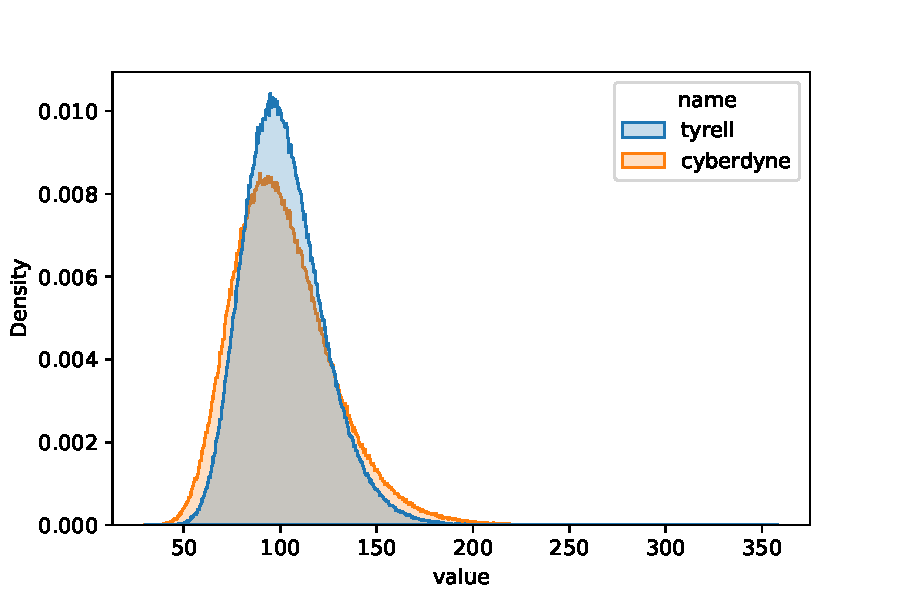
\includegraphics[scale=0.5]{hist.pdf}
\caption{Distribution of stock prices at $t=10$}
\label{plot}
\end{figure}
\end{frame}

    

\end{document}